\documentclass[a4paper,12pt]{article} % добавить leqno в [] для нумерации слева

%%% Работа с русским языком
\usepackage{cmap}					% поиск в PDF
\usepackage{mathtext} 				% русские буквы в фомулах
\usepackage[T2A]{fontenc}			% кодировка
\usepackage[utf8]{inputenc}			% кодировка исходного текста
\usepackage[english,russian]{babel}	% локализация и переносы
\usepackage[left=1cm,right=1cm,top=1cm,bottom=2cm,bindingoffset=0cm]{geometry}
\usepackage{graphicx}
\graphicspath{{img/}}
\DeclareGraphicsExtensions{.pdf,.png,.jpg}

%% Шрифты
\usepackage{euscript}	 % Шрифт Евклид
\usepackage{mathrsfs} % Красивый матшрифт

%%% Заголовок
\author{\LaTeX{} в Вышке}
\title{Гвоздарев}
\date{\today}

\begin{document} % конец преамбулы, начало документа

\begin{flushright}
\large{\textbf{Влияние атмоферы на распространение радиоволн}}
\end{flushright}

Обычно атмосферу делят на три её основных слоя: \

\begin{enumerate}

\item\textbf{Тропосфера} (от греч. trоpos — поворот, изменение и сфера), нижняя, преобладающая по массе часть земной атмосферы, в которой температура понижается с высотой. Тропосфера простирается в среднем до высот в интервале от 8 до 18 км в разных широтах. В тропосфере сосредоточено более всей массы атмосферного воздуха. Вся деятельность человека проходит в тропосфере. Самые высокие горы остаются в пределах тропосферы.

\item Над тропосферой располагается \textbf{стратосфера} (от лат. stratum - настил, слой) — слой атмосферы, располагающийся на высоте от 11 до 50 км. Характерно незначительное изменение температуры в слое 11—25 км (нижний слой стратосферы) и повышение ее в слое 25 - 40 км от \(-56,5^{\circ}С\) до \(+0,8^{\circ}\)С (верхний слой стратосферы или область инверсии). Стоит заметить, что в стратосфере расположен озоновый слой, защищающий нас от УФ лучей. Воздушный транспорт лишь частично выходит в стратосферу. 

\item Самый верхний слой атмосферы это \textbf{ионосфера}, в общем значении — слой атмосферы планеты, сильно ионизированный вследствие облучения космическими лучами. 

\end{enumerate}

Теперь стоит отметить, что по на распространение радиоволн стратосфера оказывает то же влияние, что и тропосфера, но оно проявляется в меньшей степени из-за малой плотности воздуха. Поэтому остановимся на рассмотрении двух основных слоёв. \

\begin{flushleft}
\textbf{Начнём с тропосферы:}
\end{flushleft}

Газовый состав тропосферы постоянен и идентичен сос­таву у поверхности: 78\% азота, 21\% кислорода, 0,33\% аргона, 0,03\% CO2 и т. д. Содержание водяного пара - от 0 до 4\% по объ­ёму. \

Типов радиоволн, передающиеся через тропосферу, существует целое многообразие. Например, с помощью них передаются сигналы от различных видов связи (телевидение, телеграф, телефон) и сигналы, позволяющие управлять различными системами на расстоянии (радотелемеханика). \

 В электрическом отношении тропосфера представляет собой весьма неоднородную среду, поэтому влияние тропосферы на распространение радиоволн проявляется так:

\begin{enumerate}

\item \textsl{искривляются траектории распространения раидоволн (рефракция)} \\
Явление рефракции обусловлено изменением диэлектрической проницаемости и, соответственно, показателя преломления с высотой. \\
Абсолютные изменения этих величин крайне незначительны. Несмотря на это, его достаточно для того, чтобы траектория пологого луча заметно отклонилась от прямой. \\
Кроме этого, в реальных условиях возможны также такие состояния атмосферы, когда показатель преломления возрастает с высотой. \\
Явление рефракции радиоволн в атмосфере рассматривают с позиций геометрической оптики, т.е. в основу кладут закон преломления оптических лучей. \\
Для определенности, рассматривается прохождение луча сквозь тропосферу, где показатель преломления убывает с высотой. \textbf{(Рис. 1)} В целях упрощения задачи тропосфера считается слоисто-неоднородной, составленной из отдельных участков каждый из которых характеризуется средним показателем преломления \(n_{i}\). \\
При прохождении луча из нижнего слоя в расположенный над ним следующий слой происходит отклонение луча от перпендикуляра к слою, поскольку это прохождение совершается из среды, оптически более плотной, в среду, оптически менее плотную. \\
Таким образом, проходящий из слоя в слой луч испытывает постепенный излом (отрезки красного цвета). Вследствие плавного изменения показателя преломления с увеличением высоты этот излом является плавным искривлением луча, т.е. траектория волны есть плавная линия. \\
При аномальных условиях в атмосфере (резкое увеличение давления, влажности, температуры) возможна и сверхрефракция, при которой радиоволна возвращается к Земле, отражается, и так многократно. Принято говорить, что в этом случае образуется тропосферный волновод (искусственный или естественный направляющий канал, в котором может распространяться волна). При этом в тропосфере возможно волноводное распространение радиоволн на очень большие расстояния.\\
Сверхрефракцией также обусловлено такое явление, как оптический мираж. \\
При критической рефракции дальность работы современных радиосредств значительно выше, чем при нормальной, а возникает она в том случае, если влажность
убывает с высотой также, как и при нормальной, температура меняется медленнее. 

\item \textsl{происходит рассеяние радиоволн; поглощение энергии, переносимой ими, газами атмосферы и ослабление радиоволн из-за осадков (дождь, туман, град, снег, гроза)} \\
Процесс рассеяния радиоволн можно представить себе следующим образом. Тропосфера неоднородна по своему строению, она представляет собой совокупность неустойчивых воздушных объемов — неоднородностей, в которых коэффициент преломления воздуха отличается на некоторую небольшую величину от среднего значения. Эти неоднородности непрерывно флуктуируют, т. е. их плотность, форма и размеры непрерывно меняются. Радиоволна, падающая на эти неоднородности, наводит в каждой из них токи, которые, в свою очередь, излучают примерно как антенны. Таким образом, неоднородности играют роль своеобразных ретрансляторов. \\
Основную роль в рассеянии радиоволн играют неоднородности, размеры, которых во много раз превышают длину волны. \\
При рассеянии радиоволн на каплях воды размеры неоднородностей много меньше длины волны и рассеиваемые волны распространяются равномерно во все стороны. При условиях, имеющих место в тропосфере, рассеяние происходит в пределах угла, составляющего несколько градусов с направлением падающей волны. Поэтому основная часть энергии волны проходит сквозь рассеивающую область и не может быть использована для приема. Только небольшая часть энергии возвращается на Землю, где она может быть принята. \textbf{(Рис. 2)} \\
Молекулярное поглощение в атмосфере происходит в основном на частотах близких к резонансным. Резонансные линии всех газов атмосферы, за исключением кислорода и водяного пара, расположены вне диапазона радиоволн, поэтому существенно влияет на дальность действия радиотехнических систем только поглощение молекулами кислорода и водяного пара. \\
Другой причиной, вызывающей потери энергии сигнала при распространении, является рассеяние радиоволн, прежде всего дождевыми каплями и туманом. \textbf{\textsl{Чем больше отношение "радиус капли / длина капли", тем больше потери энергии за счёт её рассеяние во всех направлениях.}}
\end{enumerate}

\begin{flushleft}
\textbf{Переходим к ионосфере:}
\end{flushleft}

Под действием радиоволны в ионосфере могут возникать как вынужденные колебания электронов и ионов. \
Существенное влияние на распространение радиоволн оказывает магнитное поле Земли, пронизывающее ионосферу. Попадающая в ионосферу волна испытывает двойное лучепреломление, т.е. расщепляется на 2 волны, отличающиеся скоростью и направлением распространения, поглощением и многими другими факторами. \
В ионосфере так же присутствуют неоднородности, от которых радиоволны отражаются. Так некоторые неоднородные образования возникают в ионосфере при вторжении в неё метеоритов. Испускаемые раскалённым метеоритом электроны ионизируют окружающую среду, образуя за летящим метеоритом след, диаметр которого вследствие молекулярной диффузии быстро возрастает. Так же радиоволны зеркально отражаются от метеорного следа. \

Радиоволны звуковых частот могут просачиваться через ионосферу вдоль силовых линий магнитного поля Земли. Распространяясь вдоль магнитной силовой линии, волна уходит на расстояние, равное нескольким земным радиусам, и затем возвращается в сопряжённую точку, расположенную в др. полушарии  \textbf{(Рис. 3)}. \

Так же существует фактор интерференции \

\textbf{Интерференция} \textbf{(Рис. 4)} проявляется вследствие многолучевого распространения. По своей природе, радиоволны могут распространяться в нескольких направлениях. В процессе многократного отражения от земной поверхности, различных препятствий, сигнал достигает места назначения разными путями. \
В месте приема, в зависимости от фазы пришедших лучей сигнал может как увеличиться (разные лучи складываются), так и уменьшиться (разные лучи компенсируют друг друга). Интерференционный характер электромагнитного поля внутри помещений (за счет многократных отражений от предметов) выражен более резко. В большей части помещений можно столкнуться и с так называемыми «мертвыми зонами», в которых прием сигнала сильно затруднен. Такая ситуация возможна, даже если передатчик и приемник находятся в прямой видимости. \
На открытой местности интерференция играет не меньшую роль, чем в помещении. На приемную антенну ВСЕГДА попадает прямая и отраженная волна, поскольку имеет место отражение от земли. На \textbf{(Рис. 5)} изображена схема путей прямой и отраженной волн от базовой станции до приемной антенны, а на графике справа на этом же рисунке уровень сигнала в зависимости от высоты для волны длиной 3см.

%Приложения
\newpage

\begin{figure}
\centering
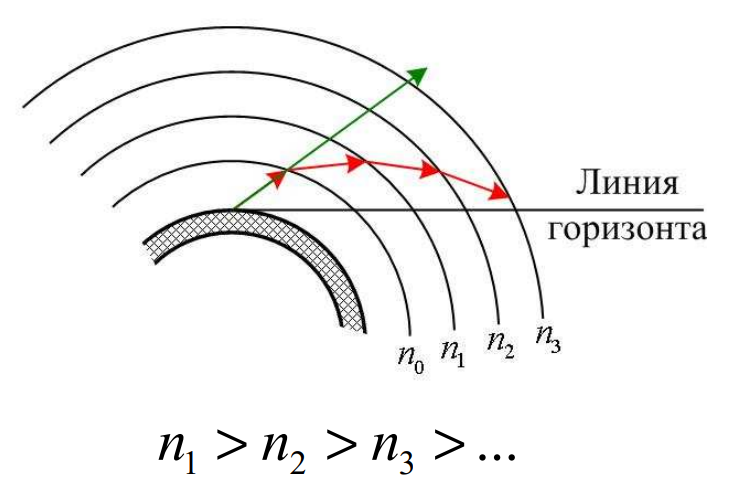
\includegraphics[width=12cm]{1. refraction}
\caption{Явление рефракции}
\end{figure}

\begin{figure}
\centering
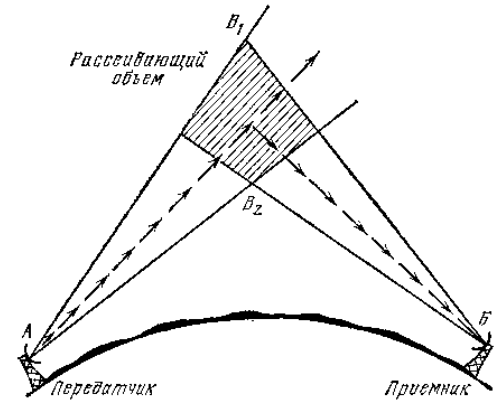
\includegraphics[width=12cm]{2. rasseianie}
\caption{Явление рассеяния}
\end{figure}

\begin{figure}
\centering
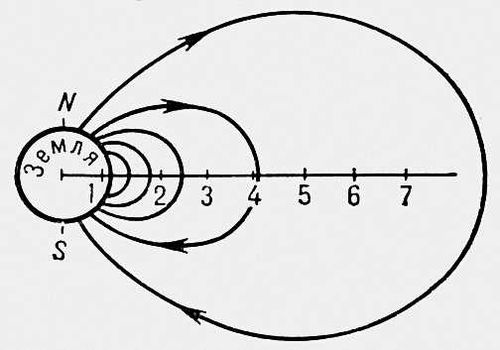
\includegraphics[width=12cm]{3. magnitpole}
\caption{Распространение радиоволн вдоль магнитной линии}
\end{figure}

\begin{figure}
\centering
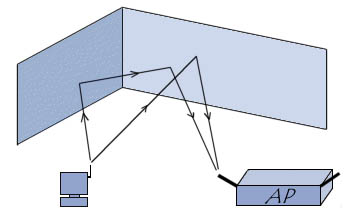
\includegraphics[width=12cm]{4. interferention}
\caption{Явление интерференции}
\end{figure}

\begin{figure}
\centering
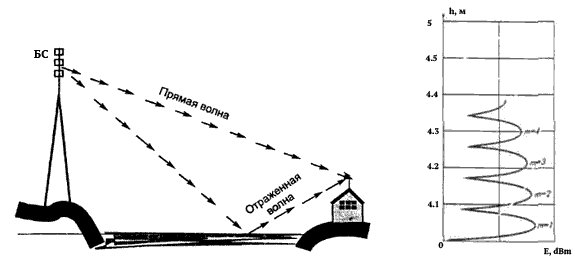
\includegraphics[width=12cm]{5. interference}
\caption{Явление интерференции}
\end{figure}

\end{document} % конец документа